\documentclass[10pt,a4paper]{article}
\usepackage[utf8]{inputenc}
\usepackage[finnish]{babel}
\usepackage[T1]{fontenc}
\usepackage{graphicx}

\usepackage{hyperref}

\begin{document}

\title{A* ja Dikstra vertailussa}
\author{Matti Nelimarkka}

\setlength{\parindent}{0pt}
\setlength{\parskip}{1ex}

\maketitle

\newpage

\section*{Tehtävänanto}

Toteuta yleinen ohjelma verkon käsittelyä varten, siten että siinä on mahdollisuus säilöä solmuja ja solmujen välisiä kaaria. Verkko tulee voida määritellä ulkoisessa tiedostossa muodossa \texttt{<solmu 1>:<solmu 2>:<etäisyys solmusta 1 solmuun 2>}, esimerkiksi:

\begin{verbatim}
a:b:5
a:c:10
a:d:1
c:b:4
d:c:10
\end{verbatim}

Lisäksi toteuta lyhyimmän polun etsintä sekä Dikstran algoritmilla \cite{dikstra} että A*-algoritmilla \cite{astar}. Vertaa näitä kahta toteutustapaa toisiinsa empiirisesti.

\section{Toteutus}

Ohjelma on toteutettu oliomallinnusta hyödyntäen: paketteja, rajapintoja ja perintäsuhteita on käytetty selkeyttämään ohjelman rakennetta. Ohjelma koostuu neljästä paketista

\begin{description}
\item[datastructures] sisältää ohjelman toiminnan kannalta välttämättömät itse toteutetut tietorakenteet kekoa, hajautustaulua ja listaa varten. Tarkemmin tätä pakettia käsitellään kappaleessa \ref{datastructures}.
\item[model] sisältää ohjelman tarvitsemat itsenäiset toteutustietorakenteet, yleisen muodon verkon sekä erityiset versiot verkosta, jotka toteuttavat tutkittava olevat Dikstran sekä A*-algoritmit. Yleistä verkkoa on esitelty tarkemmin kappaleessa \ref{model.graph} ja lyhyimmän polun etsintää kappaleessa \ref{path}.
\item[io] tarjoaa palveluja tiedoston lukemiseen tekstiformaatista ohjelman ymmärtämäksi verkoksi. Tätä käsitellään kappaleessa \ref{io}.
\item[test] sisältää ohjelman muiden luokkien testaamiseen tarvittavat luokat. Ohjelman jokaiselle luokalle on kirjoitettu yksikkötestit. Testausprosessia on käsitelty tarkemmin kappaleessa \ref{test}.
\end{description}


\subsection{Omat tietorakenteet}
\label{datastructures}

Tietorakenteiden harjoitustyön luonteen vuoksi toteutukseen on kuulunut omien tietorakenteiden kehittäminen ja testaaminen. Käytännöllisistä syistä johtuen tietorakenteeni vastaavat \texttt{java.util}-paketin tietorakenteita, koska tämä mahdollisti ketterämmän kehityksen\footnote{Muuttujat on määritelty yleisten rajapintojen kautta, jolloin niiden implementaatioluokat pystyi helposti vaihtamaan Javan rajapintaa toteuttavasta luokasta omaan toteutukseeni.} ja Javan valmiiden toiminnallisuuksien käytön osana ohjelmaa. Täsmällisesti toteutussuhteet on esitetty taulukossa \ref{omat_tietorakenteet}.

\begin{table}

\begin{tabular}{l|l}
Toteuttava luokka & Rajapinta \\ 
\hline 
\texttt{MyMap} &  \href{http://docs.oracle.com/javase/6/docs/api/java/util/Map.html}{\texttt{java.util.Map}} \\
\texttt{MyHeap} & \href{http://docs.oracle.com/javase/6/docs/api/java/util/Queue.html}{\texttt{java.util.Queue}} \\ 
\texttt{MyList} & \href{http://docs.oracle.com/javase/6/docs/api/java/util/List.html}{\texttt{java.util.List}} \\ 
\texttt{MySet} & \href{http://docs.oracle.com/javase/6/docs/api/java/util/Set.html}{\texttt{java.util.Set}} \\ 
\texttt{MyIterator} & \href{http://docs.oracle.com/javase/6/docs/api/java/util/ListIterator.html}{\texttt{java.util.ListIterator}} \\ 
\end{tabular}

On syytä huomata, että \texttt{MyHeap}-luokan \texttt{contains}-metodi eroaa esimerkiksi \href{http://docs.oracle.com/javase/6/docs/api/java/util/PriorityQueue.html}{\texttt{PriorityQueue}}-dokumentaation lupaamasta suoritusajasta $\mathcal{O}(n)$. Koska tiedämme, että sisäisen toteutuksen lista on aina järjestyksessä, on mahdollista käyttää puolitushakua, joka takaa suoritukseen ajan $\mathcal{O}(\log n)$.

\caption{Omien tietorakenteiden vastaavuus Javan tietorakenteiden kanssa}
\label{omat_tietorakenteet}
\end{table}

\subsection{Malli}
\label{model.graph}

Verkko koostuu solmuista ja solmujen välisistä kaarista, eli matemaattisemmin $\mathcal{G}( \mathbb{V}, \mathbb{E})$. Tässä ohjelmassa verkkoa vastaa luokka \texttt{Graph}, ja solmua vastaa luokka \texttt{Node}.

\texttt{Graph} koostuu listasta \texttt{Node}ja, ja kukin \texttt{Node} sisältää tiedon naapurisolmuistansa ja kaarien painoista. Verkkoon voi lisätä solmuja metodilla \texttt{addNode(Node node)} tai operaatiolla \texttt{addAll(Collection<Node> collection)}. Suoritusajat käyttäen \texttt{MyList}-luokkaa ovat vastaavasti $\mathcal{O}(1)$ ja $\mathcal{O}(n)$. Verkon solmut on saatavissa listana metodilla \texttt{edges()}, ja tämä operaatio on myös vakiaikainen, palauttaen verkon listan. Vaihtoehtoisena ratkaisuna olisi voinut käyttää sisäisessä toteutuksessa hajautustaulua verkon nimiltä verkon alkioille. Tämä olisi säilyttänyt samat suoritusajat lisäyksessä, mutta nopeuttanut hakua solmun nimen perusteella vakioaikaseksi, listan tapauksessa tämä aika on lineaarinen. Vastaavasti alkioiden käsittely listana olisi vakioaikaisen operaation sijaan $\mathcal{O}(n)$-operaatio, koska listan alkiot tulisi kerätä erikseen hajautustaulusta. Koska vakioaikainen suoritus verkon solmujen listaamiseen on tämän ohjelman kannalta keskeisempi operaatio, niin listojen käyttö oli tässä tapauksessa suositellumpi vaihtoehto.

\texttt{Node}n tehtävän on tallentaa tietoa solmun nimestä ja solmun naapureista. Solmun naapurit on tallennettu hajautustauluun, jossa on tallessa naapurisolmut ja niitä vastaavina pareina kaaren paino. Hajautustaulu on luonnollinen valinta tässä tapauksessa, koska se sallii lähes vakioaikaisen ($\mathcal{O}(1 + \frac{n}{k})$) lisäämisen, avainta vastaavan arvon noutamisen sekä avaimen arvon olemassaolon tarkistamisen. Nämä ovat keskeiset \texttt{Node}n tarjoamat ominaisuudet: uuden naapurin lisääminen (\texttt{ linkTo(Node n, double weight)}), kahden alkion välisen etäisyyden noutaminen (\texttt{linkWeight(Node n)}) sekä sen tarkistaminen, onko kahden alkion välillä kaarta (\texttt{linkTo(Node n)}).

\subsection{Lyhyimmän polun etsintä}
\label{path}

Lyhyimmän polun etsintää varten toteutettiin abstrakti luokka \texttt{ShortestPathGraph}. \texttt{ShortestPathGraph} perii \texttt{Graph}-luokan, ja laajentaa sen toimintaa kahdella metodilla.

\texttt{path(Node from, Node to)} palauttaa lyhyimmän reitin solmusta \texttt{from} solmuun \texttt{to}. Lyhin reitti palautetaan listana solmuja, mukaanlukien solmut \texttt{from} ja \texttt{to}. Metodi on abstrakti, eli se jätetään toteutettavaksi \texttt{ShortestPathGraph}in  periville aliluokille, myös sen suoritusaika riippuu reitinhakualgoritmin tehokkuudesta.

\texttt{distance(Node from, Node to)} palauttaa lyhimmän reitin pituuden solmusta \texttt{from} solmuun \texttt{to}. Se käyttää hyödykseen operaatiota \texttt{path(Node from, Node to)}, joka on myös metodin laskennallisesti vaativin osuus: lista palautetuista solmuista iteroidaan ja kunkin välin etäisyys lisätään kokonaispituuteen. Koska kahden solmun välisen etäisyyden etsiminen on vakioaikainen operaatio, on kokonaispituuden laskemisen aikavaativuus $\mathcal{O}(n')$, eli lineraarisesti suhteessa lyhyimmän polun pituuteen. Kokonaisuudessan siis on selvää, että tämä on enintään solmujen kokonaismäärän suhteen lineaarinen $\mathcal{O}(v)$. Kokonaisuudessaan kokonaispituuden laskeminen saadusta polkulistasta on minimaalinen suhteessa reitinhakualgoritmiin. Kuitenkin, tällä tavoin vältetään koodin toisteisuutta huomattavasti.

Luokkaan on lisäksi lisätty suojattu sisäluokka \texttt{QueueNode}. Tämän luokan erikoisuus on \texttt{Comparable}-rajapinnan toteutus, mikä on välttämätöntä kekorakenteen kannalta. Sisäluokkaan tallennetaan etäisyys sekä \texttt{Node}, jonka etäisyyttä käsitellään. \texttt{compareTo}-metodi vertaa tätä etäisyyttä, eli käytännössä mahdollistaa minimikeon luomisen kunkin alkion etäisyyden suhteen. \texttt{equals}-metodi taas tarkastaa, onko \texttt{Node}t samat -- mutta ei kiinnitä huomiota etäisyyteen. Koska kyseessä on suojattu sisäluokka, luokka on käytettävissä vain \texttt{ShortestPathGraph}-luokan aliluokille.

\subsubsection{Dikstran algoritmi}

\subsubsection{A*-algoritmi}

\subsection{Tiedosto-operaatiot}
\label{io}

\section{Testaus}
\label{test}

Ohjelman kukin luokka on testattu erikseen JUnit-testein. Arvio code coveragesta...

Lyhyimmän polun etsimiseen tarkoitetussa testissä käytettiin apuna kolmentoista solmun verkkoa, joka on esitetty kuvassa \ref{testiverkko}. Verkko on pääosin symmetrinen, mutta kaari solmusta 12 solmuun 11 on yksisuuntainen. Kaarien painoissa on myös luotu tilanteita, joissa tietoisesti lyhyin reitti vie enemmän askelia -- tällä on tarkoitus testata reitinhakualgoritmin toimintaa.

\begin{figure}
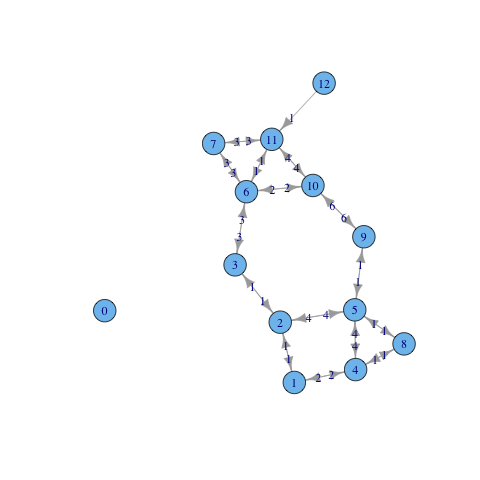
\includegraphics[scale=.5]{test_network.png} 
\caption{Lyhyimmän polun etsimiseen käytetty testiverkko}
\label{testiverkko}
\end{figure}

Täsmällisesti testit toteutettiin seuraaville tapauksille:

\begin{itemize}
\item Solmun 0 etäisyys kaikista muista solmuista tulee olla ääretön.
\item Kaikkien muiden solmujen etäisyys solmusta 0 tulee olla ääretön.
\item Etäisyys solmusta 12 solmuun 11 tulee olla 1.
\item Etäisyys solmusta 11 solmuun 12 tulee olla ääretön.
\item Lyhyin reitti solmusta 1 solmuun 5 kulkee solmujen 4 ja 8 kautta, ja muodostetun reitin pituus on 4.
\item Lyhyin reitti solmusta 5 solmuun 6 kulkee solmujen 2 ja 3 kautta, ja muodostetun reitin pituus on 8.
\item Lyhyin reitti solmusta 1 solmuun 11 kulkee solmujen 2, 3 ja 6 kautta, ja muodostetun reitin pituus on 6.
\item Lyhyin reitti solmusta 4 solmuun 5 kulkee solmun 8 kautta, ja muodostetun reitin pituus on 2.
\end{itemize}

Testit on toteutettu abstraktille yläluokalle \texttt{ShortestPathGraph}, jolloin samaa testikoodia voidaan käyttää sekä luokille \texttt{AStarPathGraph} sekä \texttt{DikstraPathGraph}.

\section{Evaluaatio}

\bibliographystyle{apalike} 
\bibliography{doc}

\end{document}